\documentclass{article}
\usepackage[left=25mm, top=20mm, right=10mm, bottom=20mm, nohead, nofoot]{geometry}
\usepackage{tabularx}
\usepackage{graphicx}
\usepackage{hyperref}
\usepackage[russian]{babel}
\usepackage[T2A]{fontenc}
\usepackage[utf8]{inputenc}

\title{Отчёт по лабораторной работе №15 по курсу «Фундаментальная информатика»}
\author{Караев Т. Ж.}
\date{25.03.23}

\begin{document}

\maketitle

\noindent
\textbf{Студент группы:} М8О-108Б-22 Караев Тариел Жоомартбекович, № по списку 11 \\
\textbf{Контакты e-mail:} \underline{idl76h@gmail.com} \\
\textbf{Работа выполнена:} «1» апреля 2023 г. \\
\textbf{Преподаватель:} асп. каф. 806 Сахарин Никита Александрович \\
\textbf{Выходной контроль знаний с оценкой:}  5 (отлично) \\
\textbf{Отчёт сдан:} «1» апреля 2023 г., \textbf{итоговая оценка} 4 (хорошо)\\
\textbf{Подпись преподавателя:} \\

\section{Тема}
Издательская система TeX

\section{Цель работы}
Получение навыков вёрстки в системе TeX

\section{Задание}
Сверстать отчёт по лабораторной работе №22

\section{Оборудование}
\textbf{Процессор:} 11th Gen Intel(R) Core(TM) i3-1115G4 @ 3.00GHz \\
\textbf{ОП:} 8 ГБ \\
\textbf{SSD:} 256 ГБ \\

\section{Программное обеспечение}
\textbf{Операционная система семейства:} Windows 11 10.0.22000 \\
\textbf{Интерпретатор команд:} Powershell 5.1.22000.832 \\
\textbf{Система программирования:} gcc.exe (GCC) 10.3.0 \\
\textbf{Текстовый редактор:} Visual Studio Code версия 1.73.1 \\
\textbf{Местонахождение и имена файлов программ и данных на домашнем компьютере:} C://Users//idl76 \\

\section{Идея, метод, алгоритм решения задачи}
1. Ознакомиться с системой TeX на лабораторном занятии. \\
2. Изучить систему по материалам лекций и источникам в интернете. \\
3. Сверстать простейший документ. \\
4. Сверстать отчёт по лабораторной работе. \\
5. Добавить в отчёт формулы, картинки, таблицы. \\
6. Конвертировать отчёт в формат pdf. \\

\section{Сценарий выполнения работы}

Математические формулы: \\
\begin{equation}
    \vec{F}=m\vec{a}
\end{equation}
\begin{equation}
    S=\frac{(v^2 - v_0^2)}{2a}
\end{equation}
\begin{equation}
    \int \frac{d x}{x^3+1}
\end{equation}

Таблица:
\begin{center}
    \begin{tabular}{|c|c|}
        \hline
         Здесь что-то написано? & Да, здесь что-то написано! \\
        \hline
         А кто это написал? & А вот это интересный вопрос... \\
        \hline
    \end{tabular}
\end{center}

Картинка:
\begin{figure}[h!]
    \centering
    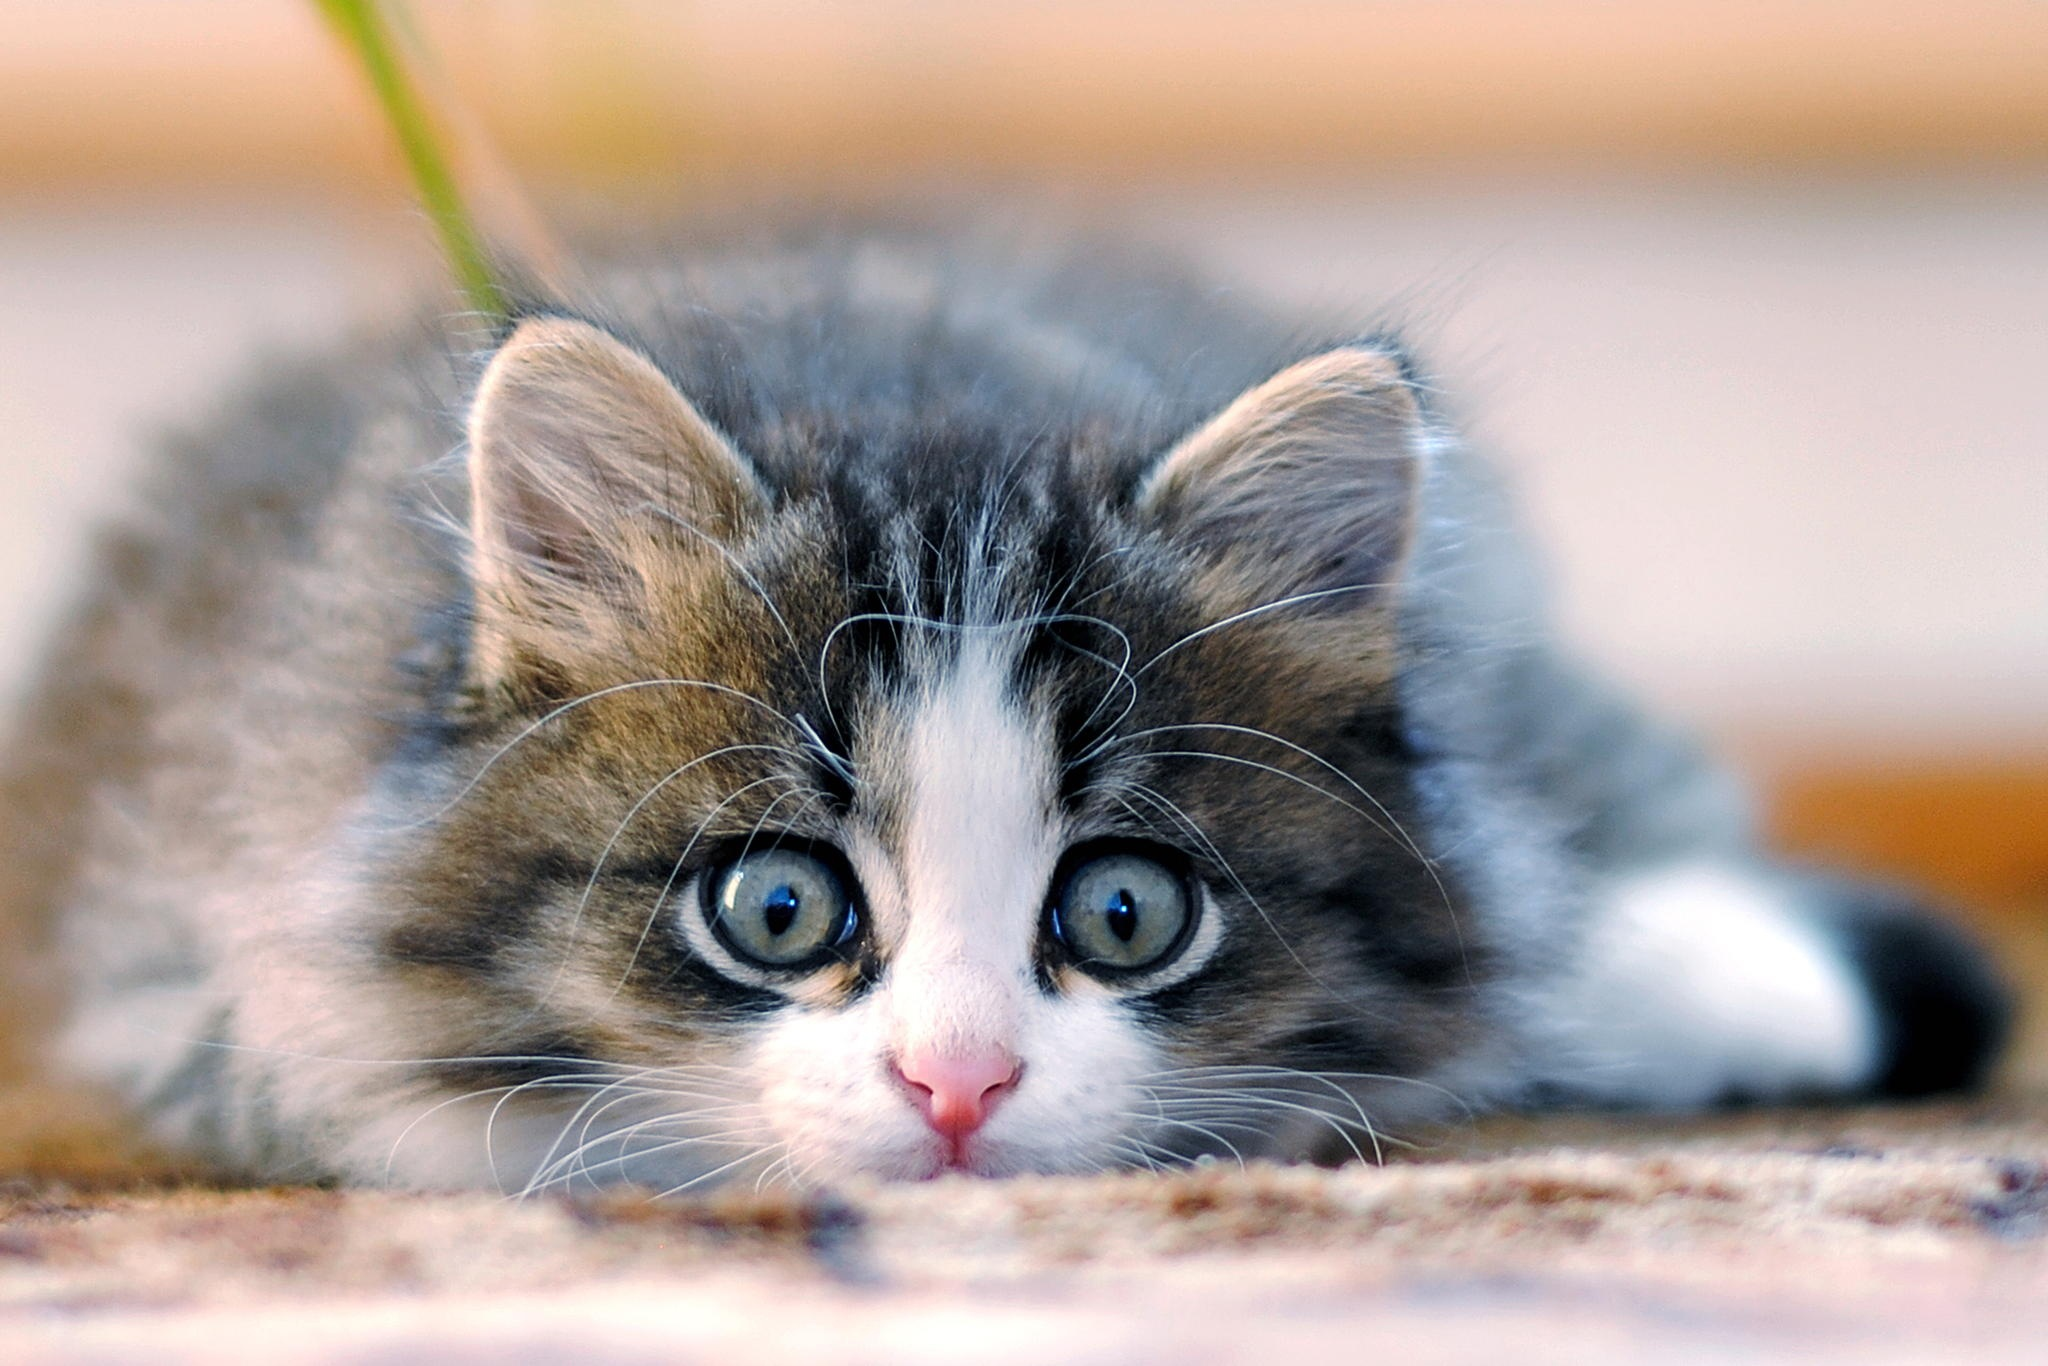
\includegraphics[width=0.8\linewidth]{cat.jpg}
    \caption{Cat}
    \label{fig:Cat}
\end{figure} \\

\section{Распечатка протокола}
\begin{verbatim}
This is pdfTeX, Version 3.141592653-2.6-1.40.24 (TeX Live 2022) (preloaded format=pdflatex 2022.8.9)  30 MAR 2023 12:53
entering extended mode
 \write18 enabled.
 %&-line parsing enabled.
**main.tex
(./main.tex
LaTeX2e <2022-06-01> patch level 5
L3 programming layer <2022-08-05> (/usr/local/texlive/2022/texmf-dist/tex/latex/base/article.cls
Document Class: article 2021/10/04 v1.4n Standard LaTeX document class
(/usr/local/texlive/2022/texmf-dist/tex/latex/base/size10.clo
File: size10.clo 2021/10/04 v1.4n Standard LaTeX file (size option)
)
\c@part=\count185
\c@section=\count186
\c@subsection=\count187
\c@subsubsection=\count188
\c@paragraph=\count189
\c@subparagraph=\count190
\c@figure=\count191
\c@table=\count192
\abovecaptionskip=\skip47
\belowcaptionskip=\skip48
\bibindent=\dimen138
) (/usr/local/texlive/2022/texmf-dist/tex/latex/geometry/geometry.sty
Package: geometry 2020/01/02 v5.9 Page Geometry
(/usr/local/texlive/2022/texmf-dist/tex/latex/graphics/keyval.sty
Package: keyval 2022/05/29 v1.15 key=value parser (DPC)
\KV@toks@=\toks16
) (/usr/local/texlive/2022/texmf-dist/tex/generic/iftex/ifvtex.sty
Package: ifvtex 2019/10/25 v1.7 ifvtex legacy package. Use iftex instead.
(/usr/local/texlive/2022/texmf-dist/tex/generic/iftex/iftex.sty
Package: iftex 2022/02/03 v1.0f TeX engine tests
))
\Gm@cnth=\count193
\Gm@cntv=\count194
\c@Gm@tempcnt=\count195
\Gm@bindingoffset=\dimen139
\Gm@wd@mp=\dimen140
\Gm@odd@mp=\dimen141
\Gm@even@mp=\dimen142
\Gm@layoutwidth=\dimen143
\Gm@layoutheight=\dimen144
\Gm@layouthoffset=\dimen145
\Gm@layoutvoffset=\dimen146
\Gm@dimlist=\toks17
) (/usr/local/texlive/2022/texmf-dist/tex/generic/babel/babel.sty
Package: babel 2022/07/20 3.78 The Babel package
\babel@savecnt=\count196
\U@D=\dimen147
\l@unhyphenated=\language87
(/usr/local/texlive/2022/texmf-dist/tex/generic/babel/txtbabel.def)
\bbl@readstream=\read2
\bbl@dirlevel=\count197
(/usr/local/texlive/2022/texmf-dist/tex/generic/babel-russian/russianb.ldf
File: russianb.ldf 2021/01/10 1.3m Russian support for the Babel system
Language: russian 2020/09/09 1.3k Russian support for the Babel system

Package babel Warning: No Cyrillic font encoding has been loaded so far.
(babel)                A font encoding should be declared before babel.
(babel)                Default `T2A' encoding will be loaded  on input line 78.

(/usr/local/texlive/2022/texmf-dist/tex/latex/cyrillic/t2aenc.def
File: t2aenc.def 2022/06/11 v1.0j Cyrillic encoding definition file
Now handling font encoding T2A ...
... processing UTF-8 mapping file for font encoding T2A
(/usr/local/texlive/2022/texmf-dist/tex/latex/base/t2aenc.dfu
File: t2aenc.dfu 2022/06/07 v1.3c UTF-8 support
   defining Unicode char U+00A4 (decimal 164)
   defining Unicode char U+00A7 (decimal 167)
   defining Unicode char U+00AB (decimal 171)
   defining Unicode char U+00BB (decimal 187)
   defining Unicode char U+0131 (decimal 305)
   defining Unicode char U+0237 (decimal 567)
   defining Unicode char U+0400 (decimal 1024)
   defining Unicode char U+0401 (decimal 1025)
   defining Unicode char U+0402 (decimal 1026)
   defining Unicode char U+0403 (decimal 1027)
   defining Unicode char U+0404 (decimal 1028)
   defining Unicode char U+0405 (decimal 1029)
   defining Unicode char U+0406 (decimal 1030)
   defining Unicode char U+0407 (decimal 1031)
   defining Unicode char U+0408 (decimal 1032)
   defining Unicode char U+0409 (decimal 1033)
   defining Unicode char U+040A (decimal 1034)
   defining Unicode char U+040B (decimal 1035)
   defining Unicode char U+040C (decimal 1036)
   defining Unicode char U+040D (decimal 1037)
   defining Unicode char U+040E (decimal 1038)
   defining Unicode char U+040F (decimal 1039)
   defining Unicode char U+0410 (decimal 1040)
   defining Unicode char U+0411 (decimal 1041)
   defining Unicode char U+0412 (decimal 1042)
   defining Unicode char U+0413 (decimal 1043)
   defining Unicode char U+0414 (decimal 1044)
   defining Unicode char U+0415 (decimal 1045)
   defining Unicode char U+0416 (decimal 1046)
   defining Unicode char U+0417 (decimal 1047)
   defining Unicode char U+0418 (decimal 1048)
   defining Unicode char U+0419 (decimal 1049)
   defining Unicode char U+041A (decimal 1050)
   defining Unicode char U+041B (decimal 1051)
   defining Unicode char U+041C (decimal 1052)
   defining Unicode char U+041D (decimal 1053)
   defining Unicode char U+041E (decimal 1054)
   defining Unicode char U+041F (decimal 1055)
   defining Unicode char U+0420 (decimal 1056)
   defining Unicode char U+0421 (decimal 1057)
   defining Unicode char U+0422 (decimal 1058)
   defining Unicode char U+0423 (decimal 1059)
   defining Unicode char U+0424 (decimal 1060)
   defining Unicode char U+0425 (decimal 1061)
   defining Unicode char U+0426 (decimal 1062)
   defining Unicode char U+0427 (decimal 1063)
   defining Unicode char U+0428 (decimal 1064)
   defining Unicode char U+0429 (decimal 1065)
   defining Unicode char U+042A (decimal 1066)
   defining Unicode char U+042B (decimal 1067)
   defining Unicode char U+042C (decimal 1068)
   defining Unicode char U+042D (decimal 1069)
   defining Unicode char U+042E (decimal 1070)
   defining Unicode char U+042F (decimal 1071)
   defining Unicode char U+0430 (decimal 1072)
   defining Unicode char U+0431 (decimal 1073)
   defining Unicode char U+0432 (decimal 1074)
   defining Unicode char U+0433 (decimal 1075)
   defining Unicode char U+0434 (decimal 1076)
   defining Unicode char U+0435 (decimal 1077)
   defining Unicode char U+0436 (decimal 1078)
   defining Unicode char U+0437 (decimal 1079)
   defining Unicode char U+0438 (decimal 1080)
   defining Unicode char U+0439 (decimal 1081)
   defining Unicode char U+043A (decimal 1082)
   defining Unicode char U+043B (decimal 1083)
   defining Unicode char U+043C (decimal 1084)
   defining Unicode char U+043D (decimal 1085)
   defining Unicode char U+043E (decimal 1086)
   defining Unicode char U+043F (decimal 1087)
   defining Unicode char U+0440 (decimal 1088)
   defining Unicode char U+0441 (decimal 1089)
   defining Unicode char U+0442 (decimal 1090)
   defining Unicode char U+0443 (decimal 1091)
   defining Unicode char U+0444 (decimal 1092)
   defining Unicode char U+0445 (decimal 1093)
   defining Unicode char U+0446 (decimal 1094)
   defining Unicode char U+0447 (decimal 1095)
   defining Unicode char U+0448 (decimal 1096)
   defining Unicode char U+0449 (decimal 1097)
   defining Unicode char U+044A (decimal 1098)
   defining Unicode char U+044B (decimal 1099)
   defining Unicode char U+044C (decimal 1100)
   defining Unicode char U+044D (decimal 1101)
   defining Unicode char U+044E (decimal 1102)
   defining Unicode char U+044F (decimal 1103)
   defining Unicode char U+0450 (decimal 1104)
   defining Unicode char U+0451 (decimal 1105)
   defining Unicode char U+0452 (decimal 1106)
   defining Unicode char U+0453 (decimal 1107)
   defining Unicode char U+0454 (decimal 1108)
   defining Unicode char U+0455 (decimal 1109)
   defining Unicode char U+0456 (decimal 1110)
   defining Unicode char U+0457 (decimal 1111)
   defining Unicode char U+0458 (decimal 1112)
   defining Unicode char U+0459 (decimal 1113)
   defining Unicode char U+045A (decimal 1114)
   defining Unicode char U+045B (decimal 1115)
   defining Unicode char U+045C (decimal 1116)
   defining Unicode char U+045D (decimal 1117)
   defining Unicode char U+045E (decimal 1118)
   defining Unicode char U+045F (decimal 1119)
   defining Unicode char U+0490 (decimal 1168)
   defining Unicode char U+0491 (decimal 1169)
   defining Unicode char U+0492 (decimal 1170)
   defining Unicode char U+0493 (decimal 1171)
   defining Unicode char U+0496 (decimal 1174)
   defining Unicode char U+0497 (decimal 1175)
   defining Unicode char U+0498 (decimal 1176)
   defining Unicode char U+0499 (decimal 1177)
   defining Unicode char U+049A (decimal 1178)
   defining Unicode char U+049B (decimal 1179)
   defining Unicode char U+049C (decimal 1180)
   defining Unicode char U+049D (decimal 1181)
   defining Unicode char U+04A0 (decimal 1184)
   defining Unicode char U+04A1 (decimal 1185)
   defining Unicode char U+04A2 (decimal 1186)
   defining Unicode char U+04A3 (decimal 1187)
   defining Unicode char U+04A4 (decimal 1188)
   defining Unicode char U+04A5 (decimal 1189)
   defining Unicode char U+04AA (decimal 1194)
   defining Unicode char U+04AB (decimal 1195)
   defining Unicode char U+04AE (decimal 1198)
   defining Unicode char U+04AF (decimal 1199)
   defining Unicode char U+04B0 (decimal 1200)
   defining Unicode char U+04B1 (decimal 1201)
   defining Unicode char U+04B2 (decimal 1202)
   defining Unicode char U+04B3 (decimal 1203)
   defining Unicode char U+04B6 (decimal 1206)
   defining Unicode char U+04B7 (decimal 1207)
   defining Unicode char U+04B8 (decimal 1208)
   defining Unicode char U+04B9 (decimal 1209)
   defining Unicode char U+04BA (decimal 1210)
   defining Unicode char U+04BB (decimal 1211)
   defining Unicode char U+04C0 (decimal 1216)
   defining Unicode char U+04C1 (decimal 1217)
   defining Unicode char U+04C2 (decimal 1218)
   defining Unicode char U+04D0 (decimal 1232)
   defining Unicode char U+04D1 (decimal 1233)
   defining Unicode char U+04D2 (decimal 1234)
   defining Unicode char U+04D3 (decimal 1235)
   defining Unicode char U+04D4 (decimal 1236)
   defining Unicode char U+04D5 (decimal 1237)
   defining Unicode char U+04D6 (decimal 1238)
   defining Unicode char U+04D7 (decimal 1239)
   defining Unicode char U+04D8 (decimal 1240)
   defining Unicode char U+04D9 (decimal 1241)
   defining Unicode char U+04DA (decimal 1242)
   defining Unicode char U+04DB (decimal 1243)
   defining Unicode char U+04DC (decimal 1244)
   defining Unicode char U+04DD (decimal 1245)
   defining Unicode char U+04DE (decimal 1246)
   defining Unicode char U+04DF (decimal 1247)
   defining Unicode char U+04E2 (decimal 1250)
   defining Unicode char U+04E3 (decimal 1251)
   defining Unicode char U+04E4 (decimal 1252)
   defining Unicode char U+04E5 (decimal 1253)
   defining Unicode char U+04E6 (decimal 1254)
   defining Unicode char U+04E7 (decimal 1255)
   defining Unicode char U+04E8 (decimal 1256)
   defining Unicode char U+04E9 (decimal 1257)
   defining Unicode char U+04EC (decimal 1260)
   defining Unicode char U+04ED (decimal 1261)
   defining Unicode char U+04EE (decimal 1262)
   defining Unicode char U+04EF (decimal 1263)
   defining Unicode char U+04F0 (decimal 1264)
   defining Unicode char U+04F1 (decimal 1265)
   defining Unicode char U+04F2 (decimal 1266)
   defining Unicode char U+04F3 (decimal 1267)
   defining Unicode char U+04F4 (decimal 1268)
   defining Unicode char U+04F5 (decimal 1269)
   defining Unicode char U+04F8 (decimal 1272)
   defining Unicode char U+04F9 (decimal 1273)
   defining Unicode char U+200C (decimal 8204)
   defining Unicode char U+2013 (decimal 8211)
   defining Unicode char U+2014 (decimal 8212)
   defining Unicode char U+2018 (decimal 8216)
   defining Unicode char U+2019 (decimal 8217)
   defining Unicode char U+201C (decimal 8220)
   defining Unicode char U+201D (decimal 8221)
   defining Unicode char U+201E (decimal 8222)
   defining Unicode char U+2030 (decimal 8240)
   defining Unicode char U+2031 (decimal 8241)
   defining Unicode char U+2116 (decimal 8470)
   defining Unicode char U+2329 (decimal 9001)
   defining Unicode char U+3008 (decimal 12296)
   defining Unicode char U+232A (decimal 9002)
   defining Unicode char U+3009 (decimal 12297)
   defining Unicode char U+2423 (decimal 9251)
   defining Unicode char U+27E8 (decimal 10216)
   defining Unicode char U+27E9 (decimal 10217)
   defining Unicode char U+FB00 (decimal 64256)
   defining Unicode char U+FB01 (decimal 64257)
   defining Unicode char U+FB02 (decimal 64258)
   defining Unicode char U+FB03 (decimal 64259)
   defining Unicode char U+FB04 (decimal 64260)
   defining Unicode char U+FB05 (decimal 64261)
   defining Unicode char U+FB06 (decimal 64262)
))
Package babel Info: Making " an active character on input line 124.
Package babel Info: Default for \cyrdash is provided on input line 163.
)) (/usr/local/texlive/2022/texmf-dist/tex/generic/babel/locale/ru/babel-russian.tex
Package babel Info: Importing font and identification data for russian
(babel)             from babel-ru.ini. Reported on input line 11.
) (/usr/local/texlive/2022/texmf-dist/tex/latex/base/fontenc.sty
Package: fontenc 2021/04/29 v2.0v Standard LaTeX package
LaTeX Font Info:    Trying to load font information for T2A+cmr on input line 112.
(/usr/local/texlive/2022/texmf-dist/tex/latex/cyrillic/t2acmr.fd
File: t2acmr.fd 2001/08/11 v1.0a Computer Modern Cyrillic font definitions
)) (/usr/local/texlive/2022/texmf-dist/tex/latex/base/inputenc.sty
Package: inputenc 2021/02/14 v1.3d Input encoding file
\inpenc@prehook=\toks18
\inpenc@posthook=\toks19
) (/usr/local/texlive/2022/texmf-dist/tex/latex/tools/tabularx.sty
Package: tabularx 2020/01/15 v2.11c `tabularx' package (DPC)
(/usr/local/texlive/2022/texmf-dist/tex/latex/tools/array.sty
Package: array 2022/03/10 v2.5f Tabular extension package (FMi)
\col@sep=\dimen148
\ar@mcellbox=\box51
\extrarowheight=\dimen149
\NC@list=\toks20
\extratabsurround=\skip49
\backup@length=\skip50
\ar@cellbox=\box52
)
\TX@col@width=\dimen150
\TX@old@table=\dimen151
\TX@old@col=\dimen152
\TX@target=\dimen153
\TX@delta=\dimen154
\TX@cols=\count198
\TX@ftn=\toks21
) (/usr/local/texlive/2022/texmf-dist/tex/latex/graphics/graphicx.sty
Package: graphicx 2021/09/16 v1.2d Enhanced LaTeX Graphics (DPC,SPQR)
(/usr/local/texlive/2022/texmf-dist/tex/latex/graphics/graphics.sty
Package: graphics 2022/03/10 v1.4e Standard LaTeX Graphics (DPC,SPQR)
(/usr/local/texlive/2022/texmf-dist/tex/latex/graphics/trig.sty
Package: trig 2021/08/11 v1.11 sin cos tan (DPC)
) (/usr/local/texlive/2022/texmf-dist/tex/latex/graphics-cfg/graphics.cfg
File: graphics.cfg 2016/06/04 v1.11 sample graphics configuration
)
Package graphics Info: Driver file: pdftex.def on input line 107.
(/usr/local/texlive/2022/texmf-dist/tex/latex/graphics-def/pdftex.def
File: pdftex.def 2020/10/05 v1.2a Graphics/color driver for pdftex
))
\Gin@req@height=\dimen155
\Gin@req@width=\dimen156
) (/usr/local/texlive/2022/texmf-dist/tex/latex/hyperref/hyperref.sty
Package: hyperref 2022-06-13 v7.00r Hypertext links for LaTeX
(/usr/local/texlive/2022/texmf-dist/tex/generic/ltxcmds/ltxcmds.sty
Package: ltxcmds 2020-05-10 v1.25 LaTeX kernel commands for general use (HO)
) (/usr/local/texlive/2022/texmf-dist/tex/generic/pdftexcmds/pdftexcmds.sty
Package: pdftexcmds 2020-06-27 v0.33 Utility functions of pdfTeX for LuaTeX (HO)
(/usr/local/texlive/2022/texmf-dist/tex/generic/infwarerr/infwarerr.sty
Package: infwarerr 2019/12/03 v1.5 Providing info/warning/error messages (HO)
)
Package pdftexcmds Info: \pdf@primitive is available.
Package pdftexcmds Info: \pdf@ifprimitive is available.
Package pdftexcmds Info: \pdfdraftmode found.
) (/usr/local/texlive/2022/texmf-dist/tex/generic/kvsetkeys/kvsetkeys.sty
Package: kvsetkeys 2019/12/15 v1.18 Key value parser (HO)
) (/usr/local/texlive/2022/texmf-dist/tex/generic/kvdefinekeys/kvdefinekeys.sty
Package: kvdefinekeys 2019-12-19 v1.6 Define keys (HO)
) (/usr/local/texlive/2022/texmf-dist/tex/generic/pdfescape/pdfescape.sty
Package: pdfescape 2019/12/09 v1.15 Implements pdfTeX's escape features (HO)
) (/usr/local/texlive/2022/texmf-dist/tex/latex/hycolor/hycolor.sty
Package: hycolor 2020-01-27 v1.10 Color options for hyperref/bookmark (HO)
) (/usr/local/texlive/2022/texmf-dist/tex/latex/letltxmacro/letltxmacro.sty
Package: letltxmacro 2019/12/03 v1.6 Let assignment for LaTeX macros (HO)
) (/usr/local/texlive/2022/texmf-dist/tex/latex/auxhook/auxhook.sty
Package: auxhook 2019-12-17 v1.6 Hooks for auxiliary files (HO)
) (/usr/local/texlive/2022/texmf-dist/tex/latex/hyperref/nameref.sty
Package: nameref 2022-05-17 v2.50 Cross-referencing by name of section
(/usr/local/texlive/2022/texmf-dist/tex/latex/refcount/refcount.sty
Package: refcount 2019/12/15 v3.6 Data extraction from label references (HO)
) (/usr/local/texlive/2022/texmf-dist/tex/generic/gettitlestring/gettitlestring.sty
Package: gettitlestring 2019/12/15 v1.6 Cleanup title references (HO)
(/usr/local/texlive/2022/texmf-dist/tex/latex/kvoptions/kvoptions.sty
Package: kvoptions 2020-10-07 v3.14 Key value format for package options (HO)
))
\c@section@level=\count199
)
\@linkdim=\dimen157
\Hy@linkcounter=\count266
\Hy@pagecounter=\count267
(/usr/local/texlive/2022/texmf-dist/tex/latex/hyperref/pd1enc.def
File: pd1enc.def 2022-06-13 v7.00r Hyperref: PDFDocEncoding definition (HO)
Now handling font encoding PD1 ...
... no UTF-8 mapping file for font encoding PD1
) (/usr/local/texlive/2022/texmf-dist/tex/generic/intcalc/intcalc.sty
Package: intcalc 2019/12/15 v1.3 Expandable calculations with integers (HO)
) (/usr/local/texlive/2022/texmf-dist/tex/generic/etexcmds/etexcmds.sty
Package: etexcmds 2019/12/15 v1.7 Avoid name clashes with e-TeX commands (HO)
)
\Hy@SavedSpaceFactor=\count268
(/usr/local/texlive/2022/texmf-dist/tex/latex/hyperref/puenc.def
File: puenc.def 2022-06-13 v7.00r Hyperref: PDF Unicode definition (HO)
Now handling font encoding PU ...
... no UTF-8 mapping file for font encoding PU
)
Package hyperref Info: Option `unicode' set `true' on input line 3130.
Package hyperref Info: Hyper figures OFF on input line 4139.
Package hyperref Info: Link nesting OFF on input line 4144.
Package hyperref Info: Hyper index ON on input line 4147.
Package hyperref Info: Plain pages OFF on input line 4154.
Package hyperref Info: Backreferencing OFF on input line 4159.
Package hyperref Info: Implicit mode ON; LaTeX internals redefined.
Package hyperref Info: Bookmarks ON on input line 4385.
\c@Hy@tempcnt=\count269
(/usr/local/texlive/2022/texmf-dist/tex/latex/url/url.sty
\Urlmuskip=\muskip16
Package: url 2013/09/16  ver 3.4  Verb mode for urls, etc.
)
LaTeX Info: Redefining \url on input line 4723.
\XeTeXLinkMargin=\dimen158
(/usr/local/texlive/2022/texmf-dist/tex/generic/bitset/bitset.sty
Package: bitset 2019/12/09 v1.3 Handle bit-vector datatype (HO)
(/usr/local/texlive/2022/texmf-dist/tex/generic/bigintcalc/bigintcalc.sty
Package: bigintcalc 2019/12/15 v1.5 Expandable calculations on big integers (HO)
))
\Fld@menulength=\count270
\Field@Width=\dimen159
\Fld@charsize=\dimen160
Package hyperref Info: Hyper figures OFF on input line 6001.
Package hyperref Info: Link nesting OFF on input line 6006.
Package hyperref Info: Hyper index ON on input line 6009.
Package hyperref Info: backreferencing OFF on input line 6016.
Package hyperref Info: Link coloring OFF on input line 6021.
Package hyperref Info: Link coloring with OCG OFF on input line 6026.
Package hyperref Info: PDF/A mode OFF on input line 6031.
(/usr/local/texlive/2022/texmf-dist/tex/latex/base/atbegshi-ltx.sty
Package: atbegshi-ltx 2021/01/10 v1.0c Emulation of the original atbegshi
package with kernel methods
)
\Hy@abspage=\count271
\c@Item=\count272
\c@Hfootnote=\count273
)
Package hyperref Info: Driver (autodetected): hpdftex.
(/usr/local/texlive/2022/texmf-dist/tex/latex/hyperref/hpdftex.def
File: hpdftex.def 2022-06-13 v7.00r Hyperref driver for pdfTeX
(/usr/local/texlive/2022/texmf-dist/tex/latex/base/atveryend-ltx.sty
Package: atveryend-ltx 2020/08/19 v1.0a Emulation of the original atveryend package
with kernel methods
)
\Fld@listcount=\count274
\c@bookmark@seq@number=\count275
(/usr/local/texlive/2022/texmf-dist/tex/latex/rerunfilecheck/rerunfilecheck.sty
Package: rerunfilecheck 2019/12/05 v1.9 Rerun checks for auxiliary files (HO)
(/usr/local/texlive/2022/texmf-dist/tex/generic/uniquecounter/uniquecounter.sty
Package: uniquecounter 2019/12/15 v1.4 Provide unlimited unique counter (HO)
)
Package uniquecounter Info: New unique counter `rerunfilecheck' on input line 286.
)
\Hy@SectionHShift=\skip51
) (/usr/local/texlive/2022/texmf-dist/tex/latex/l3backend/l3backend-pdftex.def
File: l3backend-pdftex.def 2022-08-05 L3 backend support: PDF output (pdfTeX)
\l__color_backend_stack_int=\count276
\l__pdf_internal_box=\box53
) (./output.aux)
\openout1 = `output.aux'.

LaTeX Font Info:    Checking defaults for OML/cmm/m/it on input line 14.
LaTeX Font Info:    ... okay on input line 14.
LaTeX Font Info:    Checking defaults for OMS/cmsy/m/n on input line 14.
LaTeX Font Info:    ... okay on input line 14.
LaTeX Font Info:    Checking defaults for OT1/cmr/m/n on input line 14.
LaTeX Font Info:    ... okay on input line 14.
LaTeX Font Info:    Checking defaults for T1/cmr/m/n on input line 14.
LaTeX Font Info:    ... okay on input line 14.
LaTeX Font Info:    Checking defaults for TS1/cmr/m/n on input line 14.
LaTeX Font Info:    ... okay on input line 14.
LaTeX Font Info:    Checking defaults for OMX/cmex/m/n on input line 14.
LaTeX Font Info:    ... okay on input line 14.
LaTeX Font Info:    Checking defaults for U/cmr/m/n on input line 14.
LaTeX Font Info:    ... okay on input line 14.
LaTeX Font Info:    Checking defaults for T2A/cmr/m/n on input line 14.
LaTeX Font Info:    ... okay on input line 14.
LaTeX Font Info:    Checking defaults for PD1/pdf/m/n on input line 14.
LaTeX Font Info:    ... okay on input line 14.
LaTeX Font Info:    Checking defaults for PU/pdf/m/n on input line 14.
LaTeX Font Info:    ... okay on input line 14.
*geometry* driver: auto-detecting
*geometry* detected driver: pdftex
*geometry* verbose mode - [ preamble ] result:
* driver: pdftex
* paper: <default>
* layout: <same size as paper>
* layoutoffset:(h,v)=(0.0pt,0.0pt)
* modes: 
* h-part:(L,W,R)=(71.13188pt, 514.71037pt, 28.45274pt)
* v-part:(T,H,B)=(56.9055pt, 681.15898pt, 56.9055pt)
* \paperwidth=614.295pt
* \paperheight=794.96999pt
* \textwidth=514.71037pt
* \textheight=681.15898pt
* \oddsidemargin=-1.1381pt
* \evensidemargin=-1.1381pt
* \topmargin=-15.36449pt
* \headheight=0.0pt
* \headsep=0.0pt
* \topskip=10.0pt
* \footskip=0.0pt
* \marginparwidth=65.0pt
* \marginparsep=11.0pt
* \columnsep=10.0pt
* \skip\footins=9.0pt plus 4.0pt minus 2.0pt
* \hoffset=0.0pt
* \voffset=0.0pt
* \mag=1000
* \@twocolumnfalse
* \@twosidefalse
* \@mparswitchfalse
* \@reversemarginfalse
* (1in=72.27pt=25.4mm, 1cm=28.453pt)

LaTeX Info: Redefining \th on input line 14.
(/usr/local/texlive/2022/texmf-dist/tex/context/base/mkii/supp-pdf.mkii
[Loading MPS to PDF converter (version 2006.09.02).]
\scratchcounter=\count277
\scratchdimen=\dimen161
\scratchbox=\box54
\nofMPsegments=\count278
\nofMParguments=\count279
\everyMPshowfont=\toks22
\MPscratchCnt=\count280
\MPscratchDim=\dimen162
\MPnumerator=\count281
\makeMPintoPDFobject=\count282
\everyMPtoPDFconversion=\toks23
) (/usr/local/texlive/2022/texmf-dist/tex/latex/epstopdf-pkg/epstopdf-base.sty
Package: epstopdf-base 2020-01-24 v2.11 Base part for package epstopdf
Package epstopdf-base Info: Redefining graphics rule for `.eps' on input line 485.
(/usr/local/texlive/2022/texmf-dist/tex/latex/latexconfig/epstopdf-sys.cfg
File: epstopdf-sys.cfg 2010/07/13 v1.3 Configuration of (r)epstopdf for TeX Live
))
Package hyperref Info: Link coloring OFF on input line 14.
(./output.out) (./output.out)
\@outlinefile=\write3
\openout3 = `output.out'.

LaTeX Font Info:    External font `cmex10' loaded for size
(Font)              <12> on input line 17.
LaTeX Font Info:    External font `cmex10' loaded for size
(Font)              <8> on input line 17.
LaTeX Font Info:    External font `cmex10' loaded for size
(Font)              <6> on input line 17.
LaTeX Font Info:    External font `cmex10' loaded for size
(Font)              <7> on input line 18.
LaTeX Font Info:    External font `cmex10' loaded for size
(Font)              <5> on input line 18.

Underfull \hbox (badness 10000) in paragraph at lines 18--25

 []


Underfull \hbox (badness 10000) in paragraph at lines 36--39

 []


Underfull \hbox (badness 10000) in paragraph at lines 41--46

 []


Underfull \hbox (badness 10000) in paragraph at lines 48--54

 []

[1

{/usr/local/texlive/2022/texmf-var/fonts/map/pdftex/updmap/pdftex.map}]
Underfull \hbox (badness 10000) in paragraph at lines 57--58

 []

<cat.jpg, id=58, 2055.68pt x 1371.1225pt>
File: cat.jpg Graphic file (type jpg)
<use cat.jpg>
Package pdftex.def Info: cat.jpg  used on input line 82.
(pdftex.def)             Requested size: 411.76987pt x 274.63808pt.

Underfull \hbox (badness 10000) in paragraph at lines 79--86

 []


Underfull \hbox (badness 10000) in paragraph at lines 97--97
[]|\T2A/cmr/m/n/10 Лаб. или
 []


Underfull \hbox (badness 2653) in paragraph at lines 97--97
[]|\T2A/cmr/m/n/10 Действие по
 []


Underfull \hbox (badness 10000) in paragraph at lines 97--97
[]|\T2A/cmr/m/n/10 Выполнение
 []


Underfull \hbox (badness 10000) in paragraph at lines 97--97
\T2A/cmr/m/n/10 ла-бо-ра-тор-
 []

[2 <./cat.jpg>]
LaTeX Font Info:    Trying to load font information for T2A+cmtt on input line 103.
(/usr/local/texlive/2022/texmf-dist/tex/latex/cyrillic/t2acmtt.fd
File: t2acmtt.fd 2001/08/11 v1.0a Computer Modern Cyrillic font definitions
)
Underfull \hbox (badness 10000) in paragraph at lines 101--107

 []

[3] (./output.aux)
Package rerunfilecheck Info: File `output.out' has not changed.
(rerunfilecheck)             Checksum: F955AC6F7AA502B3DEE8CE5F64682B27;2031.
 ) 
Here is how much of TeX's memory you used:
 10768 strings out of 477678
 167902 string characters out of 5829488
 489631 words of memory out of 5000000
 29422 multiletter control sequences out of 15000+600000
 477150 words of font info for 44 fonts, out of 8000000 for 9000
 1141 hyphenation exceptions out of 8191
 72i,8n,77p,458b,505s stack positions out of 10000i,1000n,20000p,200000b,200000s
{/usr/local/texlive/2022/texmf-dist/fonts/enc/dvips/cm-super/cm-super-t2a.enc}</usr/local/texlive/2022/texmf-dist/fonts/type1/public/amsfonts/cm/cmex10.pfb></usr/local/texlive/2022/texmf-dist/fonts/type1/public/amsfonts/cm/cmmi10.pfb></usr/local/texlive/2022/texmf-dist/fonts/type1/public/amsfonts/cm/cmr10.pfb></usr/local/texlive/2022/texmf-dist/fonts/type1/public/amsfonts/cm/cmr7.pfb></usr/local/texlive/2022/texmf-dist/fonts/type1/public/amsfonts/cm/cmsy10.pfb></usr/local/texlive/2022/texmf-dist/fonts/type1/public/cm-super/sfbx1000.pfb></usr/local/texlive/2022/texmf-dist/fonts/type1/public/cm-super/sfbx1440.pfb></usr/local/texlive/2022/texmf-dist/fonts/type1/public/cm-super/sfrm1000.pfb></usr/local/texlive/2022/texmf-dist/fonts/type1/public/cm-super/sfrm1200.pfb></usr/local/texlive/2022/texmf-dist/fonts/type1/public/cm-super/sfrm1728.pfb></usr/local/texlive/2022/texmf-dist/fonts/type1/public/cm-super/sftt1000.pfb>
Output written on output.pdf (3 pages, 688877 bytes).
PDF statistics:
 136 PDF objects out of 1000 (max. 8388607)
 106 compressed objects within 2 object streams
 19 named destinations out of 1000 (max. 500000)
 94 words of extra memory for PDF output out of 10000 (max. 10000000)


\end{verbatim}

\section{Дневник отладки}
\begin{center}
        \begin{tabularx}{\linewidth}{|X|X|X|X|X|X|X|}
            \hline
             № & Лаб. или дом. & Дата & Время & Событие & Действие по исправлению & Примечание \\
             \hline
             1 & дом. & 01.04.23 & 17:00 & Выполнение лабораторной работы & - & - \\
             \hline
    \end{tabularx}
\end{center}

\section{Замечания автора по существу работы}
Защита: \\
    \href{https://codeforces.com/submissions/SempaiTakoo/contest/1807}{Решённый контест}

\section{Выводы}
Была изучена система TeX и основы написания документов на этом языке программирования. Было выяснено, что за бросающимися в глаза неудобствами, вроде необходимости компилирования документа, скрывается множество достоинств и удобств. \\\\
Недочёты при выполнении задания могут быть устранены следующим образом: — \\\\
\textbf{Подпись студента:} ________________
\end{document}